\documentclass[12pt]{article}
\usepackage{amsmath,amssymb,bookmark,graphicx,parskip,pdfpages,custom}
\usepackage[margin=.8in]{geometry}
\allowdisplaybreaks
\hypersetup{colorlinks,
    citecolor=black,
    filecolor=black,
    linkcolor=black,
    urlcolor=black
}
\setcounter{secnumdepth}{5}

\begin{document}

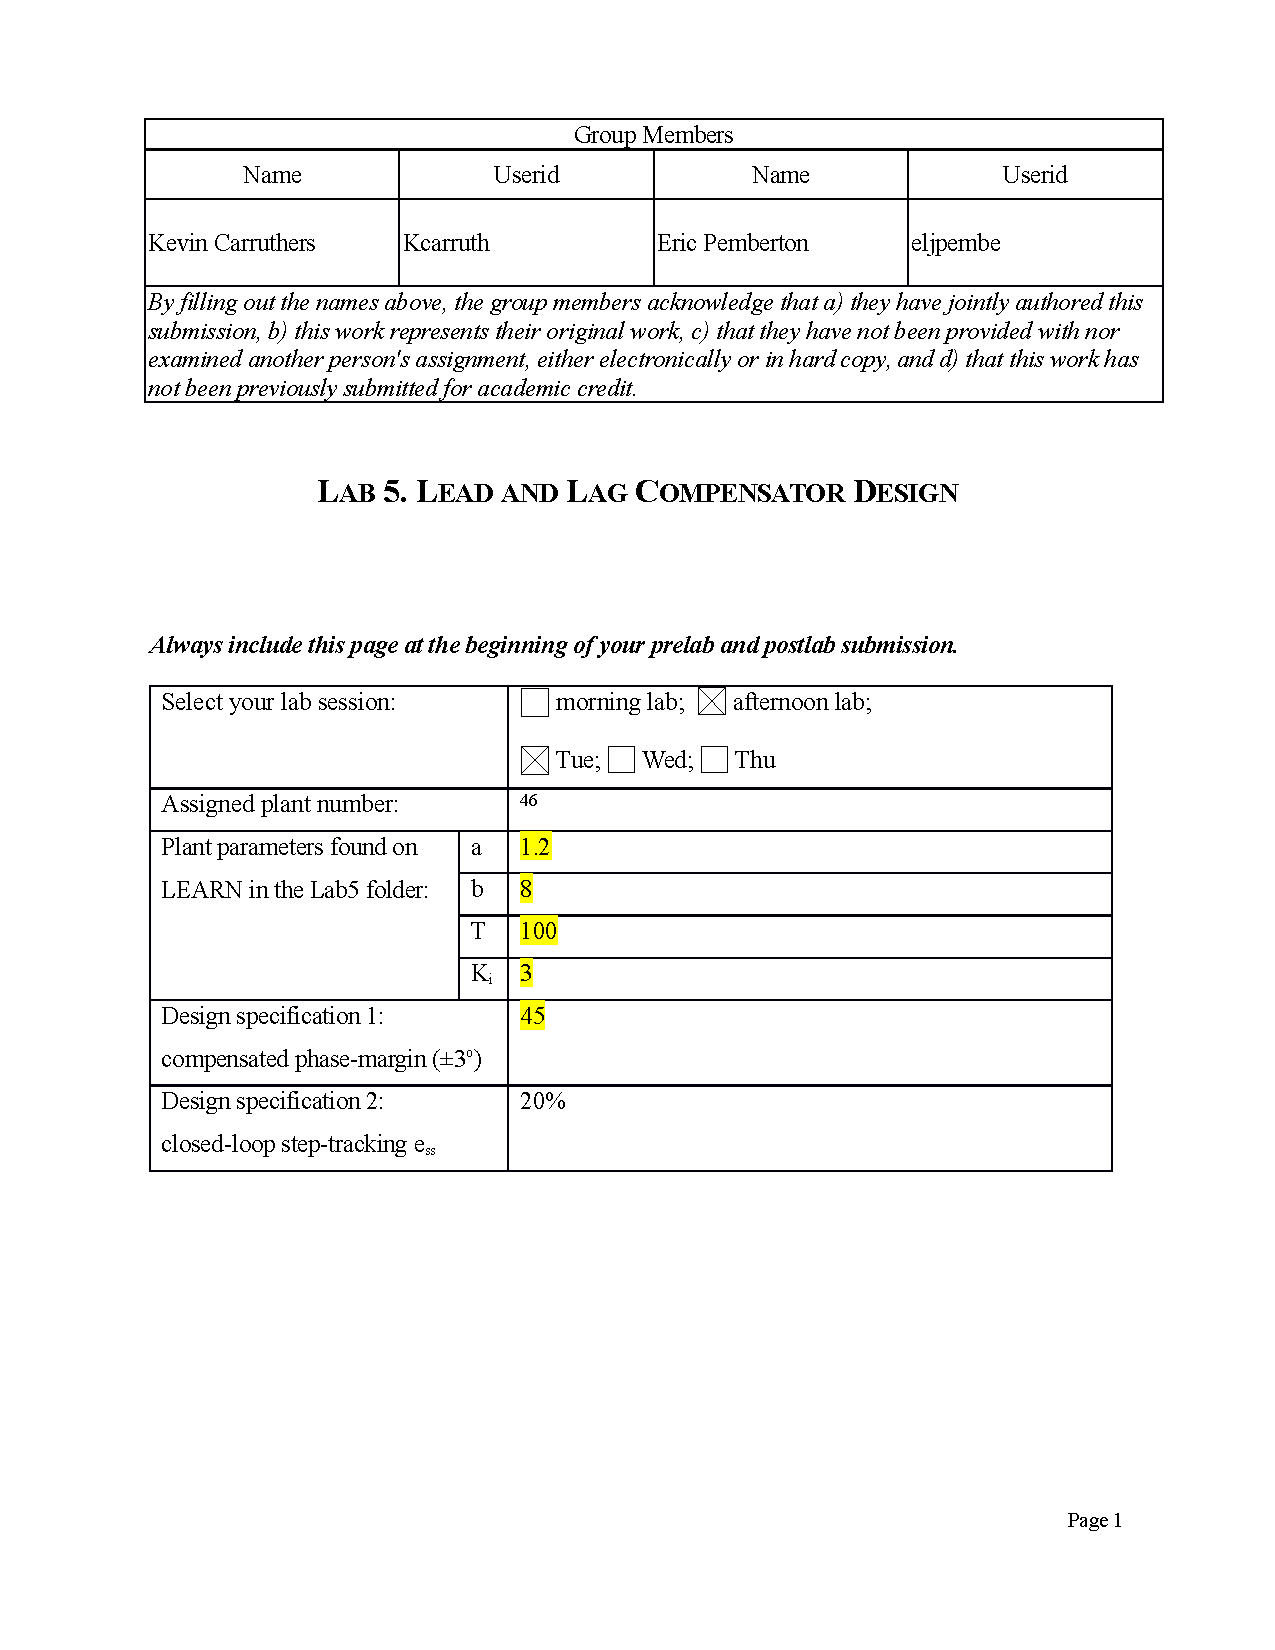
\includepdf[pages={1}]{lab5-frontpage.pdf}

\section{Question 1}
Transfer function:
\begin{align*}
P(s) &= \frac{\frac{K_i bT}{s(s + aT)}}{1 + \frac{K_i bT}{s(s + aT)}} \\
&= \frac{\frac{K_i bT}{s(s + aT)}}{\frac{s(s + aT)}{s(s + aT)} + \frac{K_i bT}{s(s + aT)}} \\
&= \frac{K_i bT}{s(s + aT) + K_i bT} \\
&= \frac{K_i bT}{s^2 + asT + K_i bT} \\
&= \frac{24000}{s^2 + 120s + 24000}
\end{align*}

Natural frequency ($\omega_n$) and damping ratio ($\zeta$): since \[ \frac{24000}{s^2 + 120s + 24000} = \frac{\omega_n^2}{s^2 + 2\zeta\omega_n s + \omega_n^2} \] we have
\begin{align*}
\omega_n^2 &= 24000 \\
\omega_n &= 40\sqrt{15} \\
2\zeta\omega_n &= 120 \\
80\sqrt{15}\zeta &= 120 \\
\zeta &= \sqrt{\frac{3}{20}}
\end{align*}

Time to first-peak ($T_p$):
\begin{align*}
T_p &= \frac{\pi}{\omega_n\sqrt{1 - \zeta^2}} \\
&= \frac{\pi}{40\sqrt{15}\sqrt{1 - \frac{3}{20}}} \\
&= \frac{\pi}{40\sqrt{15}\sqrt{\frac{17}{20}}} \\
&= \frac{\pi}{40\sqrt{\frac{51}{4}}} \\
&= \frac{\pi}{20\sqrt{51}} = 0.021996
\end{align*}

Overshoot percentage ($OS\%$):
\begin{align*}
OS\% &= e^{-\frac{\zeta\pi}{\sqrt{1 - \zeta^2}}} \\
&= e^{-\frac{\sqrt{\frac{3}{20}}\pi}{\sqrt{\frac{17}{20}}}} \\
&= e^{-\frac{\sqrt{3}\pi}{\sqrt{17}}} = 26.721\% \\
\end{align*}

Low-frequency gain:
\begin{align*}
P(j\omega) &= \frac{24000}{(j\omega)^2 + 120(j\omega) + 24000} \\
&= \frac{24000}{0^2 + 120\times 0 + 24000} \\
&= 1
\end{align*}

\section{Question 2}
What is the compensator dc-gain $K$ such that $e_{ss} \leq 20\%$.

Since this is a type-zero system, we have \[ e_{ss} = \frac{1}{1 + K_p} \] Since we wish to keep $e_{ss} \leq 20\%$, we have
\begin{align*}
\frac{1}{1 + K_p} &\leq 20\% \\
\frac{1}{1 + \lim_{s\to 0} KC(s)P(s)} &\leq 20\% \\
1 &\leq \frac{1}{5} (1 + \lim_{s\to 0} KC(s)P(s)) \\
5 &\leq (1 + \lim_{s\to 0} KC(s)P(s)) \\
4 &\leq \lim_{s\to 0} KC(s)P(s) \\
4 &\leq K
\end{align*}

So we set $K = 4$.

\section{Question 3}
We begin by drawing a Bode plot of $KP(s)$ (figure 1).
\begin{figure}[ht]
\centering
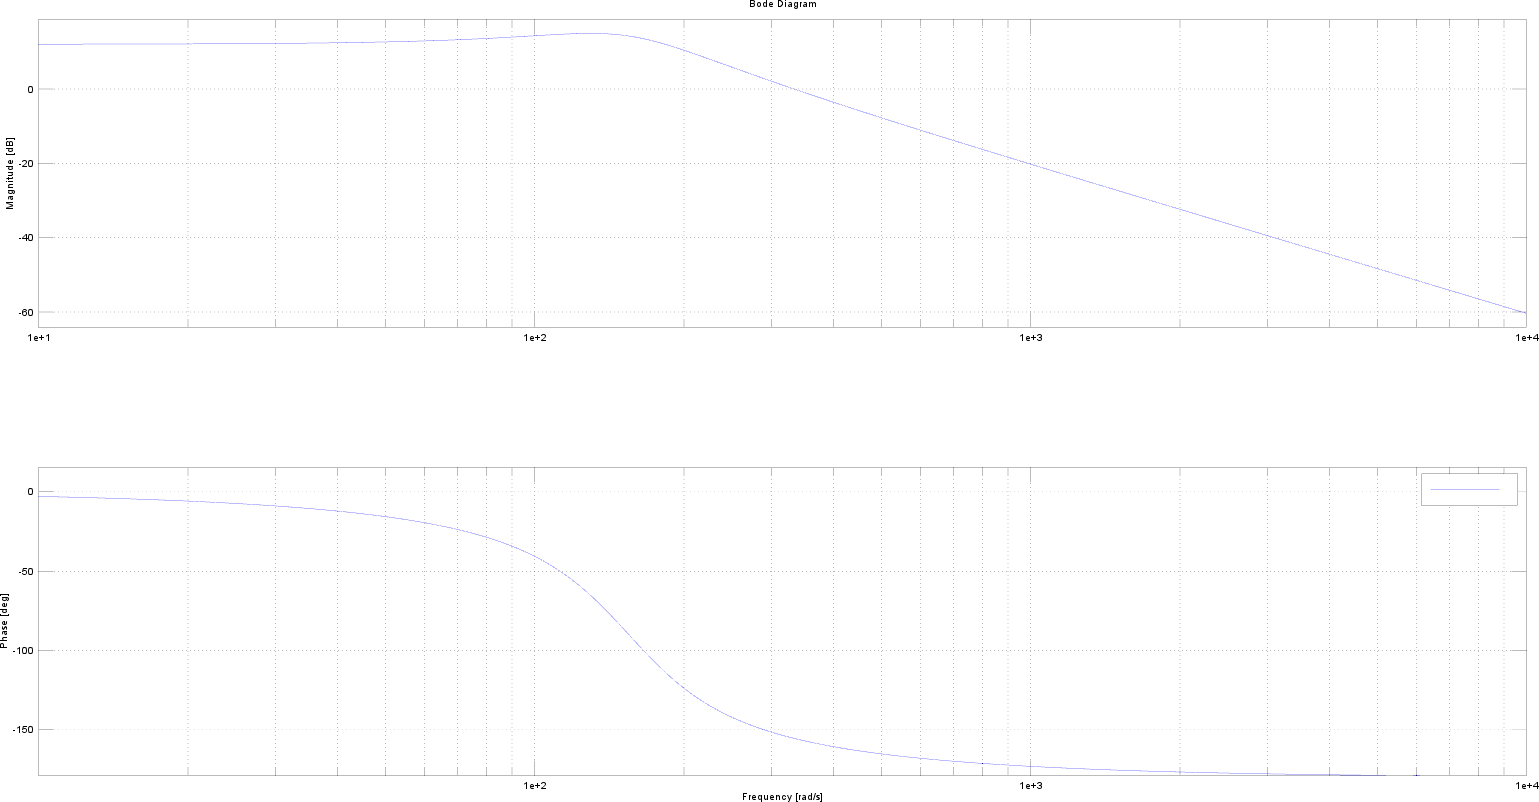
\includegraphics[width=0.8\textwidth]{lab5-bode.png}
\caption{Bode Plot of $KP(s)$}
\end{figure}

We examine this plot to find the frequency at which our phase margin exists, eg. the frequency at which the phase diagram shows a PM of $45^\circ$; this is $222.6$ rad/s, so we set $\omega_{max} = 222.6$.

The magnitude of our system at $\omega_{max}$ is $8.12$ dB. Thus we set
\begin{align*}
20\log_{10}\alpha &= -8.12 \\
\alpha &= 0.39264
\end{align*}

We can then solve for $\tau$ with
\begin{align*}
\frac{10}{\alpha\tau} &= \omega_{max} \\
\frac{10}{0.39264\tau} &= 222.6 \\
\tau &= 0.11441
\end{align*}

We thus have the transfer function \[ C(s) = \frac{0.044922s + 1}{0.11441s + 1} \] which we can simplify to \[ C(s) = \frac{0.39264s + 8.7405}{s + 8.7405} \] This gives us a zero of $-22.2608$ and a pole of $-8.7405$.

\section{Question 4}
Given $KC(s)P(s) = 4 \times \frac{0.39264s + 8.7405}{s + 8.7405} \times \frac{24000}{s^2 + 120s + 24000}$, we have \[ KC(s)P(s) = \frac{37694s + 839090}{s^3 + 128.741s^2 + 25048.9s + 209772} \]

We then get the frequency response shown in figure 2 and the step response shown in figure 3.

\begin{figure}[ht]
\centering
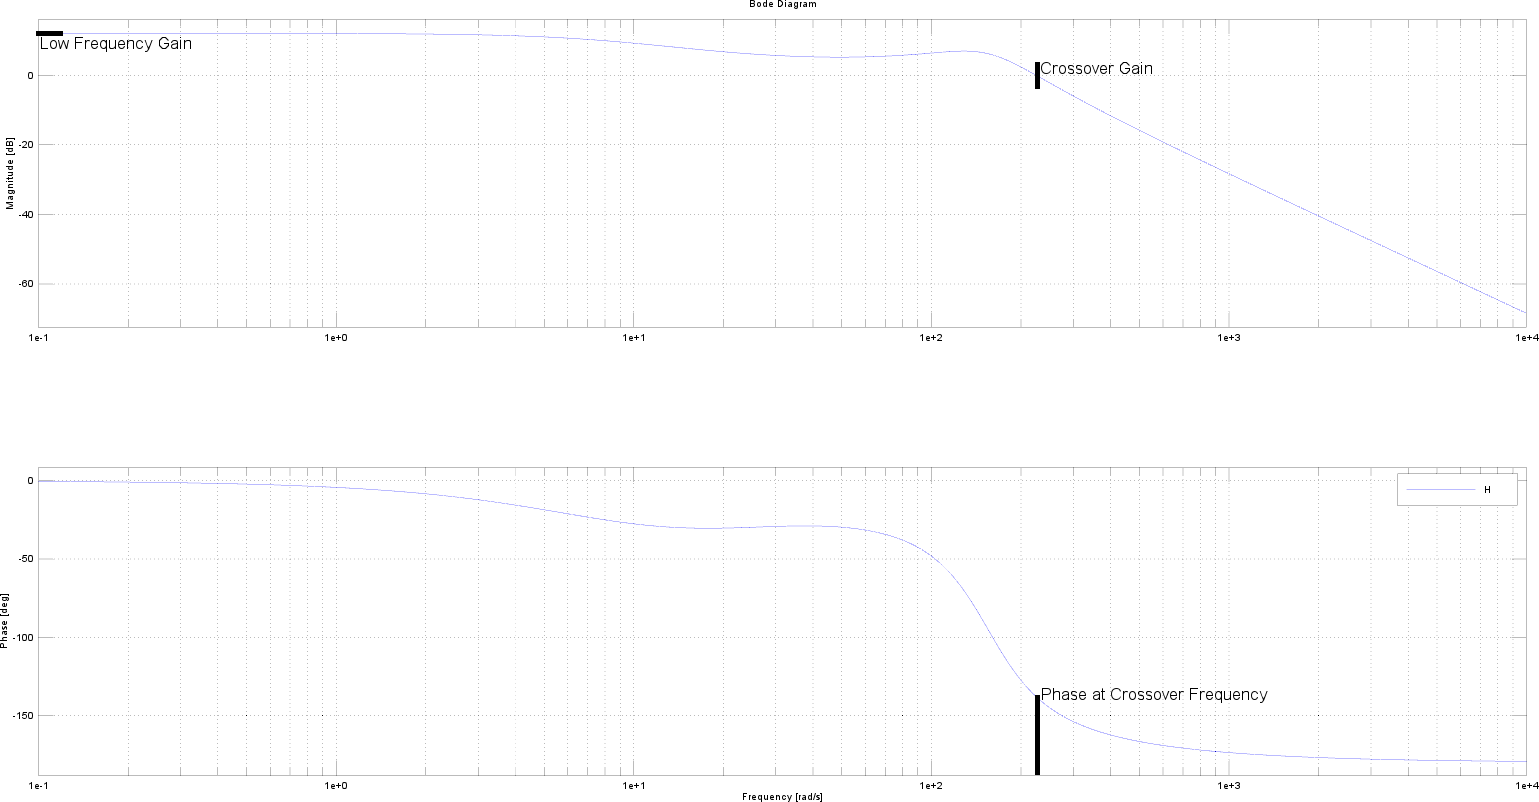
\includegraphics[width=0.8\textwidth]{lab5-lag-bode.png}
\caption{Bode Plot of $KCP(s)$ for Lag Compensated System}
\end{figure}

\begin{figure}[ht]
\centering
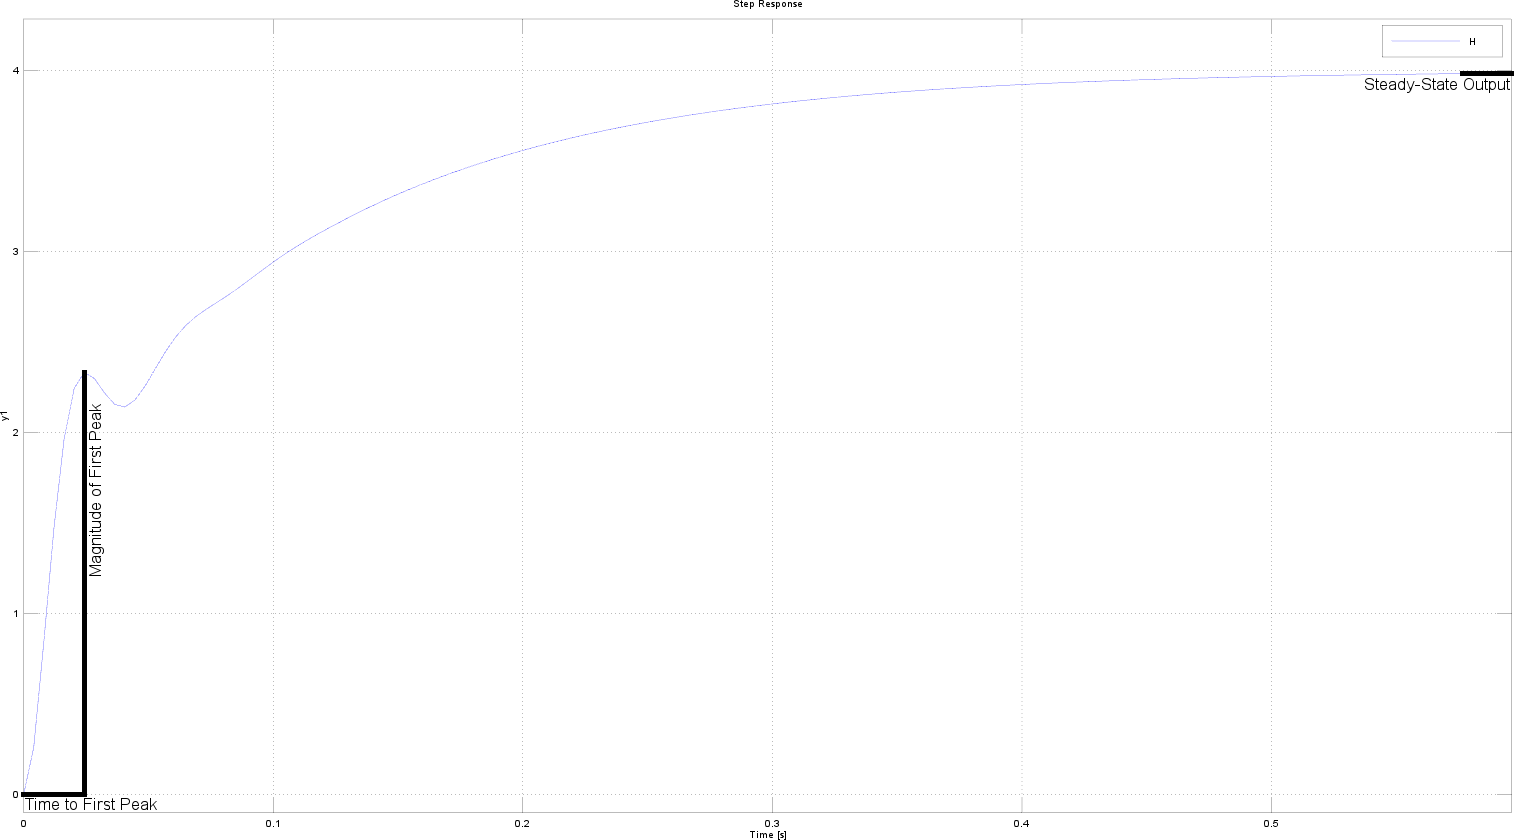
\includegraphics[width=0.6\textwidth]{lab5-lag-step.png}
\caption{Step Response of $KCP(s)$ for Lag Compensated System}
\end{figure}

\section{Question 5}
We begin by drawing a Bode plot of $KP(s)$ (figure 4).
\begin{figure}[ht]
\centering
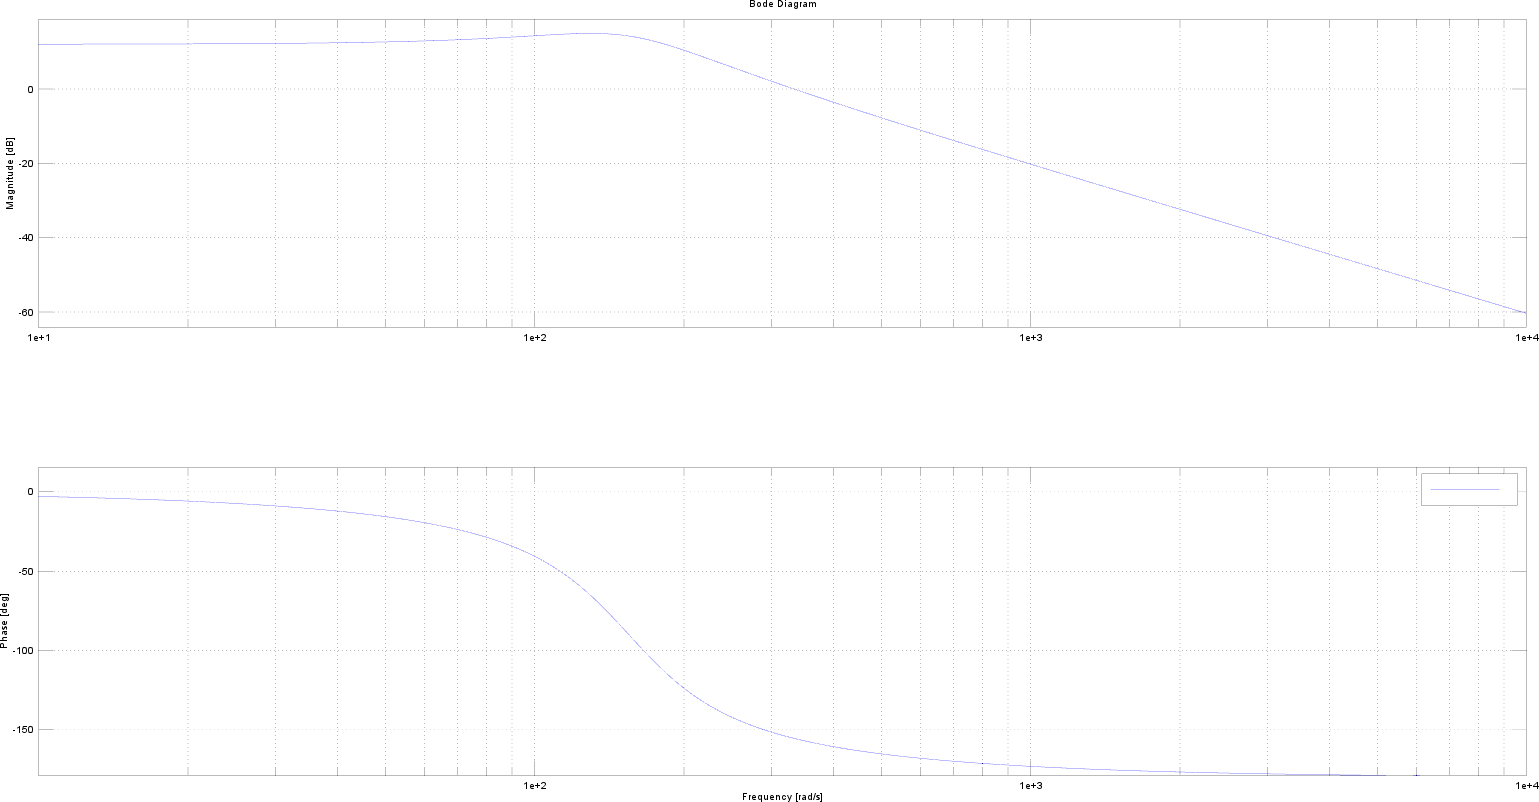
\includegraphics[width=0.8\textwidth]{lab5-bode.png}
\caption{Bode Plot of $KP(s)$}
\end{figure}

We examine this plot to find the phase margin at our $\omega_{max}$ frequency; our $\omega_{max}$ is $333.4$ rad/s, so we find our phase margin $x = |-155.8 - (-180)| = 24.2^\circ$.

We thus find $\alpha$ as
\begin{align*}
PM - x &= \sin^{-1} \frac{\alpha - 1}{\alpha + 1} \\
(45 - 24.2)^\circ &= \sin^{-1} \frac{\alpha - 1}{\alpha + 1} \\
20.8^\circ &= \sin^{-1} \frac{\alpha - 1}{\alpha + 1} \\
\alpha &= 2.101
\end{align*}

We can then solve for $\tau$ with
\begin{align*}
\omega_{max} &= \frac{1}{\sqrt{\alpha}\tau} \\
333.4 &= \frac{1}{\sqrt{2.101}\tau} \\
333.4\sqrt{2.101}\tau &= 1 \\
\tau &= \frac{1}{333.4\sqrt{2.101}} \\
\tau &= 0.0020693
\end{align*}

We thus have the transfer function \[ C(s) = \frac{0.0043476s + 1}{0.0020693s + 1} \] which we can simplify to \[ C(s) = \frac{2.101s + 483.26}{s + 483.26} \] This gives us a zero of $-230.014$ and a pole of $-483.26$.

\section{Question 6}
Given $KC(s)P(s) = 4 \times \frac{2.101s + 483.26}{s + 483.26} \times \frac{24000}{s^2 + 120s + 24000}$, we have \[ KC(s)P(s) = \frac{201696s + 46392000}{s^3 + 603.26s^2 + 81991.2s + 11598200} \]

We then get the frequency response shown in figure 5 and the step response shown in figure 6.

\begin{figure}[ht]
\centering
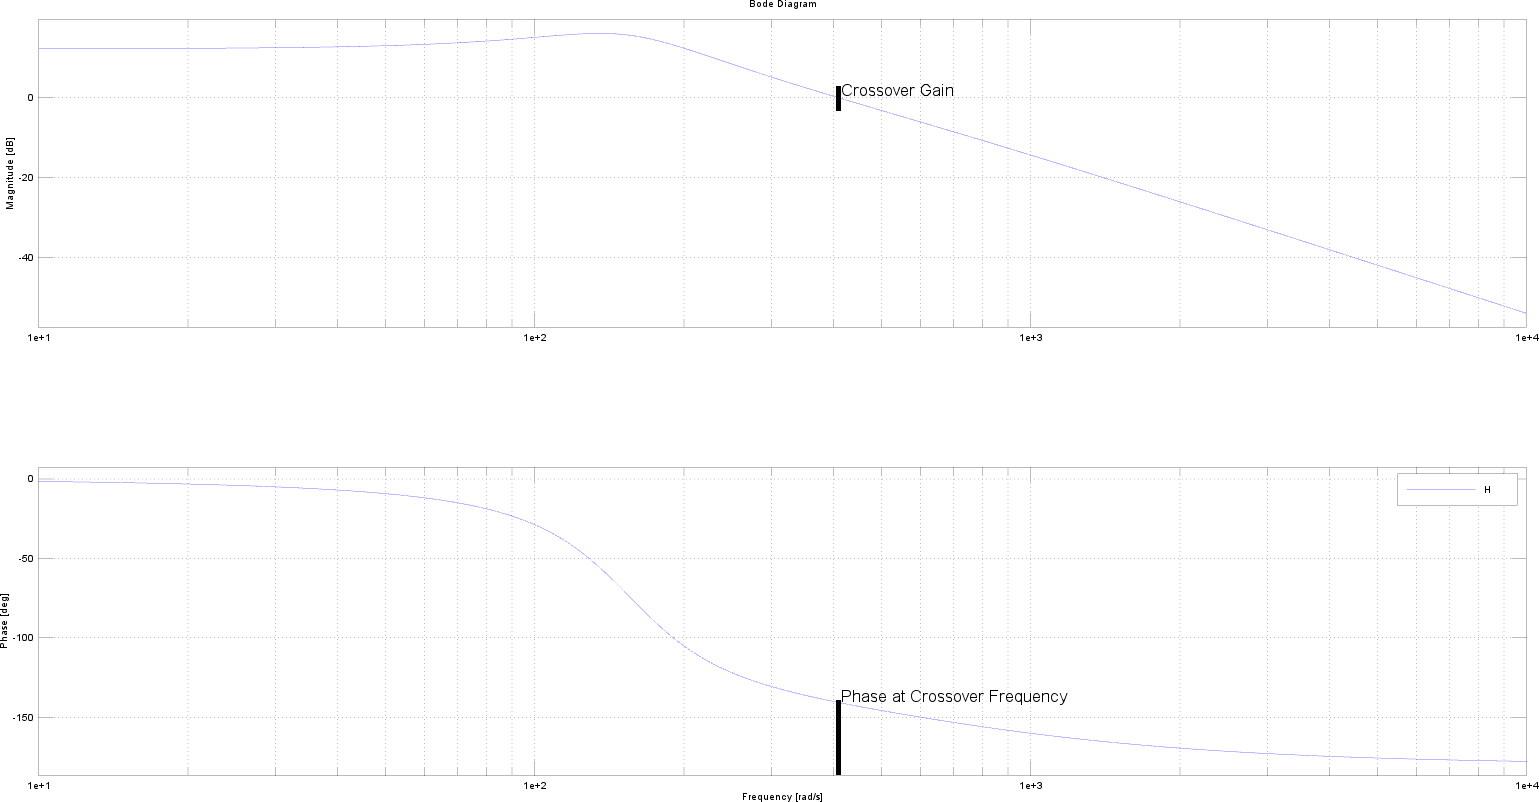
\includegraphics[width=0.8\textwidth]{lab5-lead-bode.png}
\caption{Bode Plot of $KCP(s)$ for Lead Compensated System}
\end{figure}

\begin{figure}[ht]
\centering
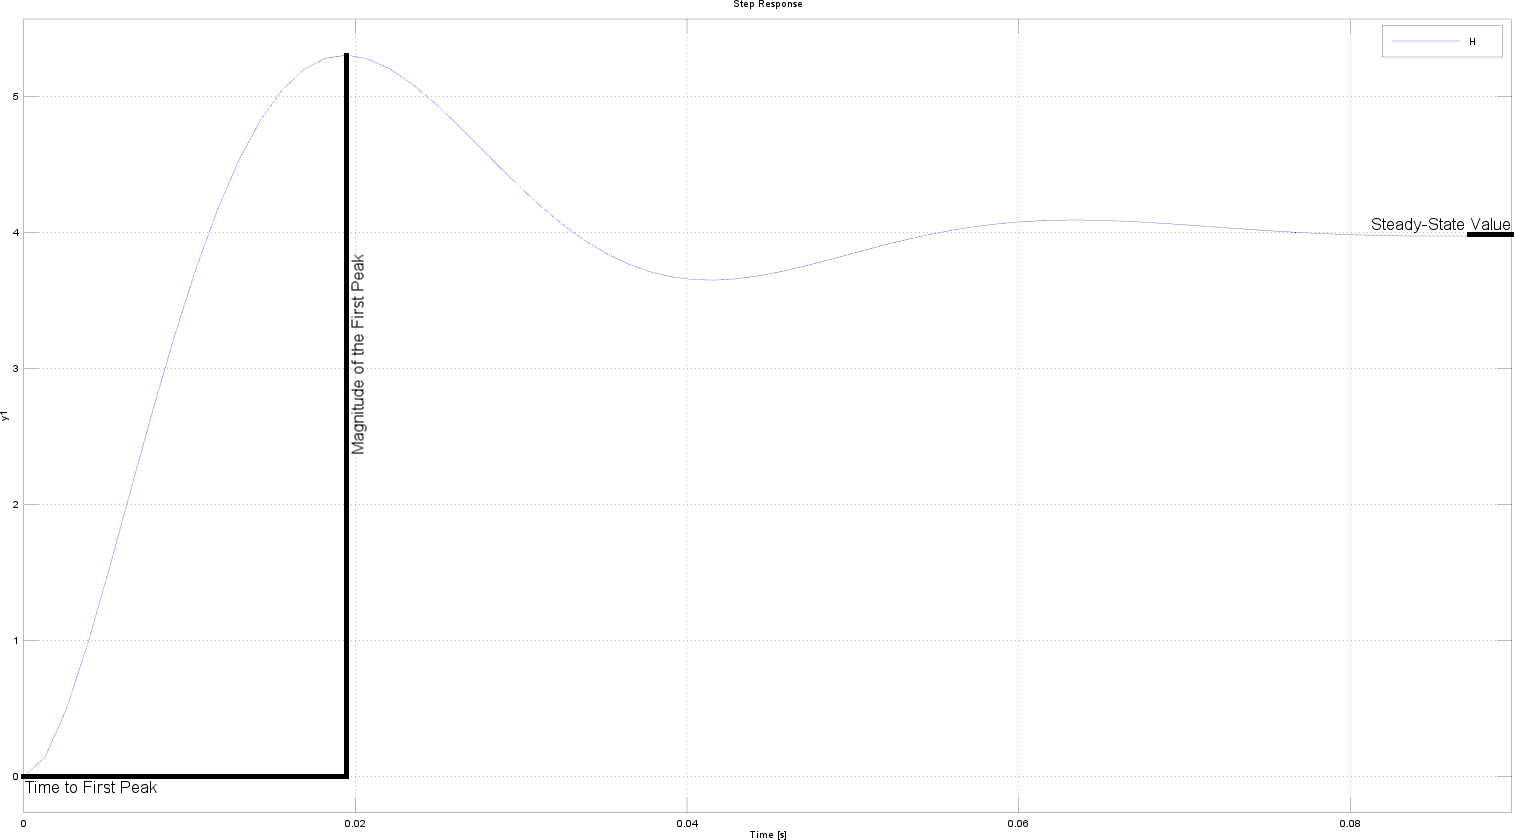
\includegraphics[width=0.6\textwidth]{lab5-lead-step.png}
\caption{Step Response of $KCP(s)$ for Lead Compensated System}
\end{figure}

\end{document}
